\documentclass[12pt,a5paper]{article}
\usepackage[cp1250]{inputenc}
\usepackage{czech}
\usepackage{amsmath,amssymb}
\usepackage[top=2cm, bottom=2cm, left=2cm, right=2cm, landscape]{geometry}

\usepackage{array}
\usepackage{multirow}
%\usepackage{amsthm,array,multirow}
\usepackage{graphicx}
%\usepackage[center]{subfigure}

\usepackage{paralist}
%\usepackage{caption}
\usepackage{verbatim} %multiline comments
%\usepackage{fancyhdr}
\usepackage{url}
%\usepackage{setspace} %double space...
%\usepackage{pdfpages} %inserting pdf

\setlength{\parskip}{1ex plus 0.5ex minus 0.2ex}


\begin{document}

\section*{Úvod}
Teorie her je matematická disciplína, která analyzuje široké spektrum konfliktních rozhodovacích situací, které mohou nastat kdekoliv, kde dochází ke střetu zájmů. Herně-teoretické modely se pak snaží tyto konfliktní situace nejen analyzovat, ale sestavením matematického modelu daného konfliktu a pomocí výpočtů se snaží nalézt co nejlepší strategie pro konkrétní účastníky takových konfliktů.

\section{Reprezentace hry}
Hra je charakterizována dvěma nebo více hráči, množinami akcí (tahů), které tito hráči mohou vykonat v určitých okamžicích, a možnými zisky, kterých hráči mohou dosáhnout. Zisk každého hráče nezávisí pouze na jím vykonaných akcích, ale také na akcích ostatních hráčů. Formálněji, existuje několik odlišných herních reprezentací: \emph{normální forma} (neboli \emph{strategická forma}), \emph{extenzivní forma} či \emph{kooperativní forma} (neboli \emph{forma charakteristické funkce}). Každé přináší jiný popis hry, a slouží tak k~různým účelům. Hra v~extenzivní formě může být využita ke specifikaci hry v~normální formě a hra v~normální formě může být použita k~definici hry v~kooperativní formě, nikoliv však naopak.

\subsection{Klasifikace her}
Rozlišujeme statické a dynamické hry. U~statických her vykonávají hráči své tahy současně, případně neznají zvolené tahy protihráčů. U~dynamických her hráči táhnou postupně, a mohou tedy reagovat na předchozí tahy protihráčů. Podle toho, zda každý z~hráčů zná zisky všech hráčů ve všech možných výsledcích hry, rozlišujeme hry s~úplnými a neúplnými informacemi.
   
Na základě tohoto členění klasifikujeme hry do čtyř skupin:
\begin{compactitem}
\item statické hry s úplnými informacemi,
\item dynamické hry s úplnými informacemi,
\item statické hry s neúplnými informacemi,
\item dynamické hry s neúplnými informacemi.
\end{compactitem}

U~her s~neúplnými informacemi pracujeme s~pravděpodobnostními rozděleními, kterými se řídí zisky protihráčů. Zde se budeme zabývat hrami s~úplnými informacemi.
 
\subsection{Statické hry a normální forma}
\emph{Strategie} hráče je kompletní plán akcí, který specifikuje, jaké tahy má hráč vykonat v~závislosti na dosavadním průběhu hry. V~případě statických her pojmy akce a strategie splývají. 

Ke specifikaci statických her s~úplnými informacemi slouží normální forma.

%\fbox{
%\parbox{.8\textwidth}{
\emph{Hra v normální formě} obsahuje následující prvky:
\begin{compactitem}
\item množinu hráčů: $\{1,\dots , n\}$,
\item množinu strategií $S_i$ pro každého hráče $i \in \{1,\dots , n\}$,
\item výplatní funkci $u_i : S_1 \times \dots \times S_n \rightarrow \mathbb{R}$ pro každého hráče $i \in \{1,\dots , n\}$.
\end{compactitem}
%}}

Hra dvou hráčů v normální formě je nejčastěji charakterizována pomocí \emph{dvojmatice}.

\begin{figure}[htb]
\centering
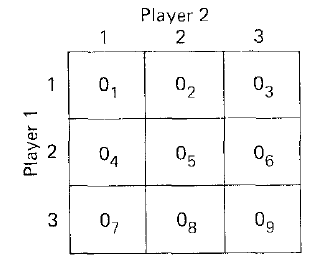
\includegraphics[scale=0.35]{1_3.png}
\caption{Hra v normální formě v podobě dvojmatice \label{bimatrix}}
\end{figure}

Normální forma může být použita i~k~popisu dynamických her. Je však třeba specifikovat, kdy je který hráč na tahu, jaké akce může vykonat a jaké informace má o~dosavadním průběhu hry. Pojmy akce a strategie se u~dynamických her rozcházejí. Definujme nejprve extenzivní formu.

\emph{Příklad:} Vězňovo dilema

\subsection{Extenzivní forma}
Extenzivní forma reprezentace hry specifikuje:
\begin{compactitem}
\item množinu hráčů,
\item kdy je který hráč na tahu,
\item jaké má hráč informace o dosavadním průběhu hry ve chvíli, kdy je hráč na tahu,
\item množinu akcí, které může hráč podstoupit,
\item výplatní funkci každého hráče jakožto funkci akcí podstoupených všemi hráči. 
\end{compactitem}

Jako první popsali hru pomocí extenzivní formy von Neumann a Morgenstern (1944) a poté Kuhn (1953). V~obou případech se jednalo o~konečné hry, tj. hry, ve kterých je konečný počet hráčů, tahů i akcí. Příkladem takových her jsou např. šachy nebo poker. Nicméně málokteré situace v ekonomice či politice jsou modelovány konečnými hrami. 

Hra v extenzivní formě je nejčastěji zobrazována pomocí stromu. Jednoduchý trh v~prostředí duopolu je ilustrován Kuhnovým herním stromem. Jedná se o zjednodušený případ, kdy si každá ze dvou firem musí vybrat jednu ze tří možných úrovní produkce. Firmy se rozhodují současně. Jejich úrovně produkce určují tržní výstup a zisky obou firem. Na obrázku \ref{Kuhn} je popis této hry v extenzivní formě. Každý uzel reprezentuje stav, ve kterém se hra může nacházet (z~pohledu nezávislého pozorovatele). Hra začíná v~kořeni stromu (označeným $R$). Každý uzel, který není listem, je označen $P_i$, což indikuje, že je na tahu hráč $i$ a má na výběr z~tahů odpovídajícím větvím stromu vycházejícím z~tohoto uzlu. Listy stromu jsou označeny $O_j$ a reprezentují všechny možné výsledky hry. Každá cesta z~kořene do listu určuje možný průběh hry.

\begin{figure}[htb]
\centering
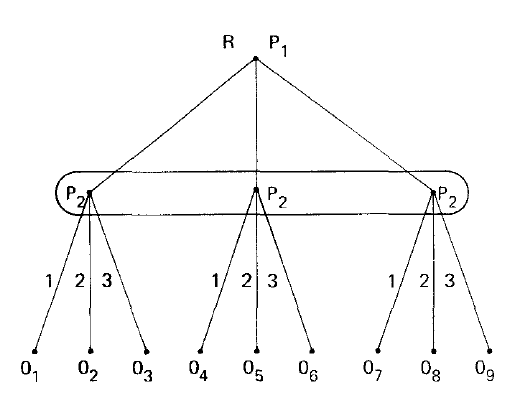
\includegraphics[scale=0.35]{1_1.png}
\caption{Kuhnův herní strom \label{Kuhn}}
\end{figure}

V~mnoha situacích můžeme vyžadovat, aby hráči táhli současně (statické hry). Nezajímá nás, zda hráči táhli přesně ve stejném okamžiku, podstatné je to, že hráči v~okamžiku rozhodnutí o~svém tahu nemají informace o~tahu protihráčů. Nezáleží na tom, kdo táhne první, protože ostatní nejsou informováni. Tuto situaci znázorňujeme ve stromě tak, že propojíme (oválem či čárkovanou čarou) všechny uzly, o~nichž hráč neví, ve kterém z~nich se nachází. Tyto uzly tvoří tzv. \emph{informační množinu}. Ze všech uzlů jedné informační množiny musí vycházet stejné hrany. Extenzivní forma tedy umožňuje reprezentovat i statické hry. Obrázky \ref{bimatrix} a \ref{Kuhn} reprezentují tutéž hru v~normální a v~extenzivní formě.

V~některých případech je třeba do hry zahrnout exogenní nejistotu. V~takové situaci přidáme do hry dalšího hráče $P_0$, nazývaného \emph{Příroda}. Kdykoliv je tento hráč na tahu, s~danými pravděpodobnostmi vybere jednu z větví. Příklad hry obsahující \emph{Přírodu} je na obrázku \ref{nature}.

\begin{figure}[htb]
\centering
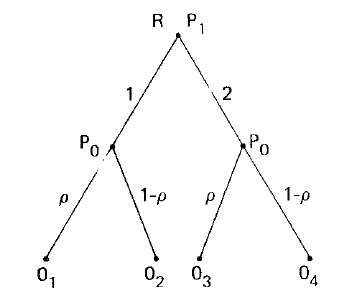
\includegraphics[scale=0.35]{1_2.png}
\caption{ Hra obsahující hráče \emph{Příroda} \label{nature}}
\end{figure}

Hry, které obsahují pouze jednoprvkové informační množiny se nazývají hry s~\emph{perfektními informacemi}. Takovou hrou jsou šachy. V~každém okamžiku hry znají všichni hráči všechny detaily cesty z~kořene do současného uzlu. To neplatí pro poker, či pro aukce s~uzavřenými nabídkami.

V~terminologii stromů a informačních množin můžeme \emph{strategii} definovat jako funkci, která každé informační množině hráče přiřadí jednu z~alternativ (tj. hran) vycházejících z~této informační množiny. 

\subsection{Dynamické hry a normální (strategická) forma}
Dynamické hry je možné také reprezentovat v~normální formě. Nyní ovšem rozlišujeme pojmy akce a strategie. V~záhlavích tabulky (resp. dvojmatice) nyní již nebudou akce, ale kombinace akcí, přesněji strategie.

Uvažujme modifikaci hry v~extenzivní formě na obrázku~\ref{Kuhn}. Nahraďme informační množinu hráče $P_2$ dvěma informačními množinami, a to tak, že pokud hráč $P_1$ zvolí možnost 1, $P_2$ je informován, zvolí-li $P_1$ možnost 2 nebo 3, $P_2$ neví, ve kterém z~těchto dvou uzlů se nachází. Tato hra je v~normální formě reprezentována maticí $3 \times 9$, protože existuje 9 různých strategií pro $P_2$. Strategiemi hráče $P_2$ jsou uspořádané dvojice $(i,j)$, $i,j \in \{1,2,3\}$, které chápeme: \uv{jestliže $P_1$ hrál 1, hraj $i$, jinak hraj $j$}. 

\subsection{Kooperativní (koaliční) forma}
V~normální formě je kladen důraz na jedince, a to v~tom smyslu, že zisk hráče závisí na jím zvolené strategii a na strategiích zvolených ostatními hráči. Není přikládán význam možnostem spolupráce mezi hráči. Při studiu tvorby kartelů, mezinárodního obchodu, vyjednávání nebo jiných skupinových jevů může být kladen důraz na možné zisky ze spolupráce mezi jednotlivými účastníky. 

Uvažujme následující hru dvou hráčů v normální formě (jedná se o obecné vězňovo dilema), $a_i > b_i > c_i > d_i$.

\begin{figure}[htb]
\centering
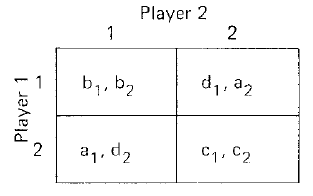
\includegraphics[scale=0.35]{1_4.png}
\caption{ Obecné vězňovo dilema v~normální formě \label{prisoner}}
\end{figure}

%Můžeme rozlišit dvě různé formy této hry, a to v~závislosti na tom, zda přijmeme předpoklad o~přenositelnosti užitku.

Označme $\upsilon(S)$ zisk, kterého může dohromady dosáhnout koalice hráčů $S$, pokud hrají jako jeden hráč. $\upsilon$ nazýváme \emph{charakteristická funkce}. Je to funkce z~podmnožin všech hráčů do reálných čísel. Pro hru $n$ hráčů existuje $2^n-1$ neprázdných koalic.

Označení $\upsilon(\overline{ij})$ je použito ke specifikaci konkrétní koalice sestávající z~hráčů $i$ a $j$. Charakteristická funkce pro vězňovo dilema na obrázku~\ref{prisoner} je následující:
\begin{gather*}
\upsilon(\emptyset)=0, \quad \upsilon(\overline{1})=c_1, \quad \upsilon(\overline{2})=c_2\\
\upsilon(\overline{12})=\max \{ (b_1+b_2),(a_1+d_2),(a_2+d_1), \}.
\end{gather*}

Charakteristická funkce může být považována za počáteční řešení hry v~tom smyslu, že její výpočet poskytne náhled do struktury hry. V~tomto příkladě byly hodnoty spočteny jako odpovědi na otázku, jakého maximálního zisku může koalice dosáhnout za předpokladu, že ostatní hráči se snaží tento zisk minimalizovat. Nejlepší, co může udělat sám hráč $P_1$, resp. $P_2$, je hrát druhou strategii a získat $c_1$, resp. $c_2$. Dohromady mohou hráči získat $b_1+b_2$. V~tomto příkladě je oprávněné vyhodnotit $\upsilon(\overline{1})$ jako $c_1$, protože hráč $P_2$ tím, že minimalizuje zisk hráče $P_1$, současně optimalizuje své vlastní skóre. To nemusí být pravda obecně, jako protipříklad slouží následující hra.

\begin{figure}[htb]
\centering
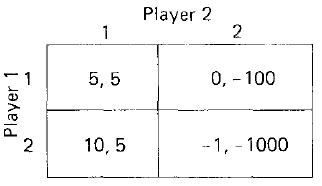
\includegraphics[scale=0.35]{1_5.png}
\caption{}
\end{figure}
 
 Zde charakteristická funkce nabývá hodnot
\[
\upsilon(\emptyset)=0, \quad \upsilon(\overline{1})=0, \quad \upsilon(\overline{2})=5, \quad
\upsilon(\overline{12})=15.
\]

Zde je poněkud nelogické považovat pozici  hráče $P_2$ za nejvýhodnější. Paradox je v~zacházení s~hrozbami. Výpočet charakteristické funkce pro hráče $P_1$ nebere v~úvahu vysoké náklady hráče $P_2$ spojené s~výběrem strategie 2.

Můžeme definovat \emph{zobecněnou charakteristickou funkci} (či \emph{charakterizující funkci}) $V(S)$, která pro každou množinu hráčů $S$ určuje množinu optimálních dosažitelných zisků.

Způsob definice zobecněné charakteristické funkce je ilustrován na obrázku \ref{charfce}, který zobrazuje příklad se třemi hráči. Osy $\alpha_1,\alpha_2,\alpha_3$ znázorňují zisky obdržené po řadě hráči 1, 2 a 3. Zacházíme s $V(S)$, jako by to byl válec, který vyřízne část Paretovsky optimální plochy pro hru $n$ hráčů jako celek. Například koalice $\overline{12}$ může získat alespoň tolik, kolik se jí dostává v~libovolném bodě části Paretovsky optimální množiny $ABC$ ohraničené $EFC$.

\begin{figure}[htb]
\centering
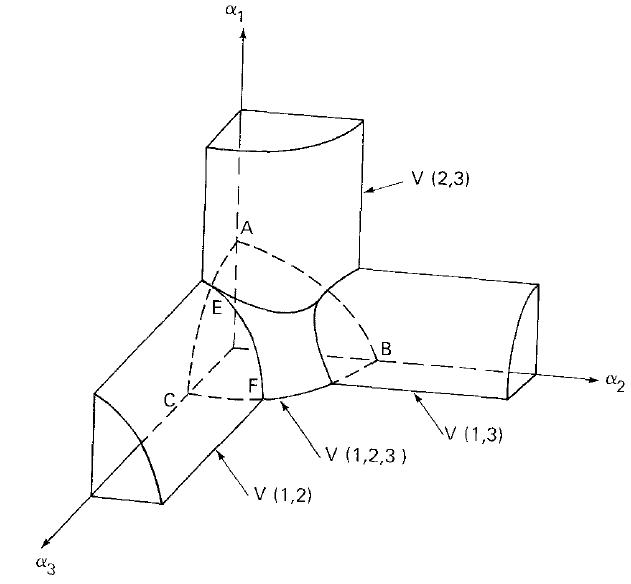
\includegraphics[scale=0.35]{1_6.png}
\caption{Zobecněná charakteristická funkce \label{charfce}}
\end{figure}
\end{document}